%!TEX root = ../tesis.tex
\section{Identificación de los focos de dengue}
\label{sec:solucion-instantanea}
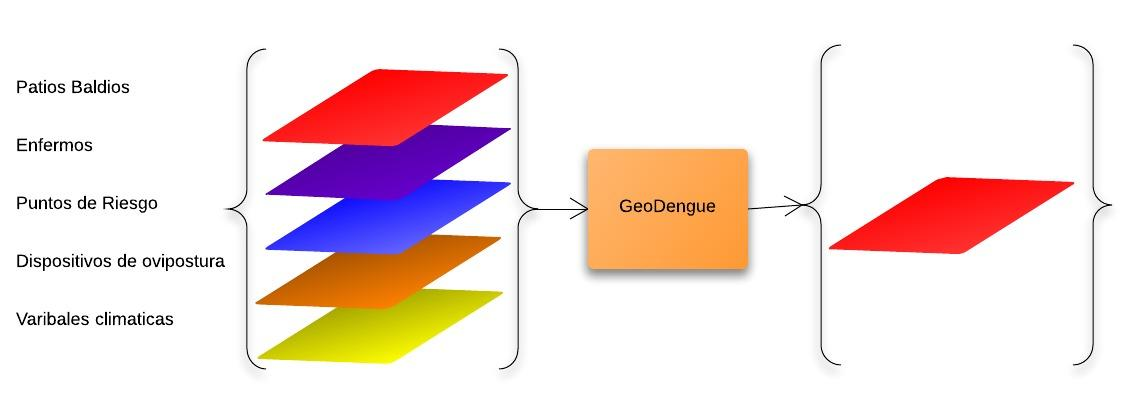
\includegraphics[ scale=0.35]{./graphics/modelo-base.jpeg}

Mediante técnicas de interpolación espacial los datos de entrada serán procesados y representados en la zona de estudio como polígonos que representan focos de la enfermedad.

Los focos se determina según los valores conocidos de las larvitrampas mediante interpolación, esto representa un instante \cite{AnusuyaSpeech20097}.
